\chapter{Estado del arte}
\label{cap:capitulo3}

\begin{flushright}
\begin{minipage}[]{10cm}
\emph{\guillemotleft A collection of files that is installed on a host to alter the standard functionality of the host in a malicious and stealthy way.\guillemotright}\\
\end{minipage}\\

NIST CSRC, \textit{Rootkit - Glossary}~\cite{nist_rootkit}.\\
\end{flushright}

A partir de la definición expuesta y de lo mencionado en la introducción de la memoria, un \textit{rootkit} es un tipo de \textit{malware} diseñado para ocultar y manipular recursos del sistema, como procesos, ficheros, conexiones de red o mecanismos de persistencia.
Su peligrosidad no reside únicamente en la escalada de privilegios que puede alcanzar, sino en su capacidad para falsear la visión del estado real de la máquina, comprometiendo la fiabilidad de su monitorización.\\

En sistemas \textit{Linux}, los \textit{rootkits} pueden clasificarse principalmente en dos grandes categorías según la capa en la que operen:\\

\begin{figure}[h!]
  \centering
  \scalebox{0.84}{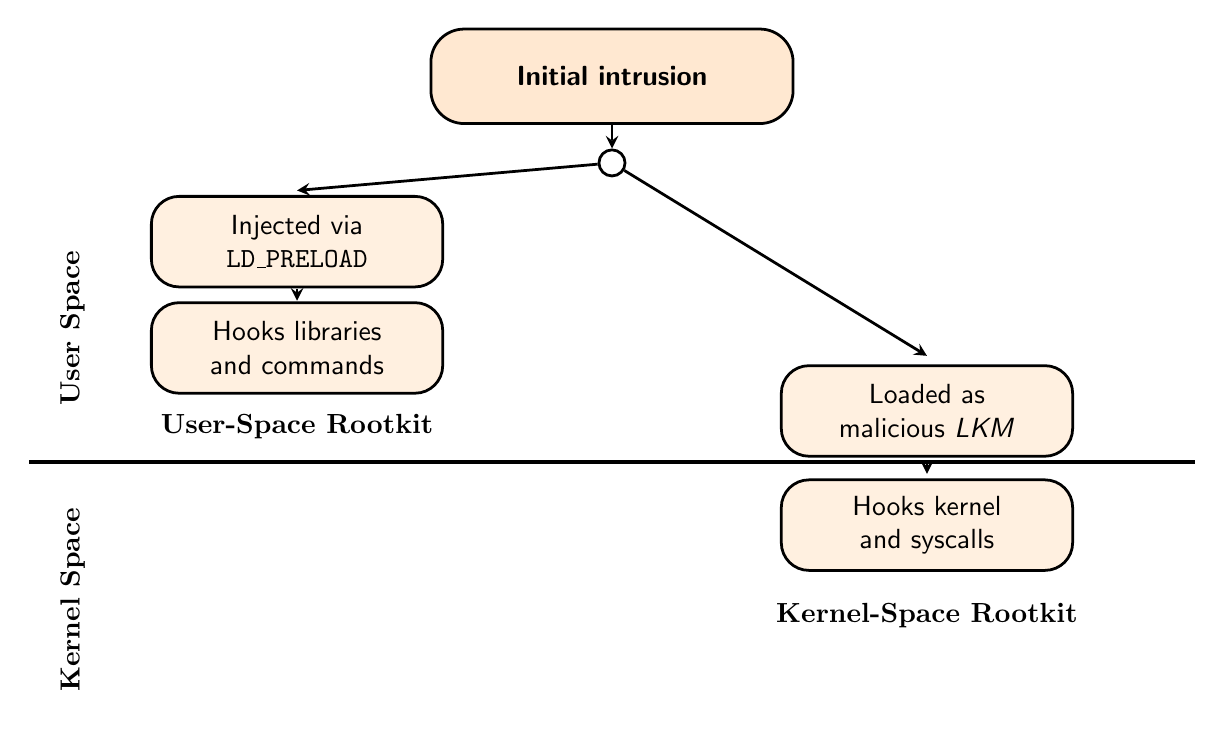
\begin{tikzpicture}[
    font=\sffamily,
    >=stealth,
    box/.style={
        draw=black,
        rounded corners=10pt,
        line width=1pt,
        align=center,
        minimum width=3.7cm,
        minimum height=1.15cm,
        fill=orange!12
    },
    boxdark/.style={
        draw=black,
        rounded corners=10pt,
        line width=1pt,
        align=center,
        minimum width=3.9cm,
        minimum height=1.15cm,
        fill=orange!28
    },
    titlebox/.style={
        draw=black,
        rounded corners=12pt,
        line width=1pt,
        align=center,
        minimum width=4.6cm,
        minimum height=1.2cm,
        fill=orange!18
    }
]

\node[titlebox] (entry) at (0,4.1) {\bfseries Initial intrusion};
\node[circle, draw=black, line width=1pt, fill=white, minimum size=0.18cm] (split) at (0,3.0) {};

\node[box] (u1) at (-4.0,2.0) {Injected via\\\texttt{LD\_PRELOAD}};
\node[box] (u2) at (-4.0,0.65) {Hooks libraries\\and commands};

\node[box] (k1) at (4.0,-0.15) {Loaded as\\malicious \textit{LKM}};
\node[box] (k2) at (4.0,-1.6) {Hooks kernel\\and syscalls};

\draw[line width=1.2pt] (-7.4,-0.8) -- (7.4,-0.8);
\node[rotate=90, font=\bfseries] at (-6.85,0.9) {User Space};
\node[rotate=90, font=\bfseries] at (-6.85,-2.55) {Kernel Space};

\draw[->, line width=1pt] (entry) -- (split);

\draw[->, line width=1pt] (split) -- (-4.0,2.65);
\draw[->, line width=1pt] (-4.0,1.4) -- (-4.0,1.25);

\draw[->, line width=1pt] (split) -- (4.0,0.55);
\draw[->, line width=1pt] (4.0,-0.8) -- (4.0,-0.95);
\node[font=\bfseries] at (-4.0,-0.35) {User-Space Rootkit};
\node[font=\bfseries] at (4.0,-2.75) {Kernel-Space Rootkit};

\end{tikzpicture}
}
  \figsource{Elaboración propia.}
  \caption{Clasificación general de \textit{rootkits} en sistemas \textit{Linux}.}
  \label{fig:rootkits_types}
\end{figure}

\section{Rootkits de Espacio de Usuario}
\label{sec:user_rootkits}

Los \textit{rootkits} de \textit{Espacio de Usuario} actúan sobre programas, bibliotecas dinámicas y herramientas de usuario del sistema operativo.
Su técnica más habitual consiste en aprovechar el mecanismo de enlazado dinámico \texttt{LD\_PRELOAD} para cargar bibliotecas de forma maliciosa y así interceptar funciones (\textit{hooking}) de uso común (como las de \texttt{libc}),
alterando de esta forma el comportamiento de comandos como \texttt{ps}, \texttt{ls}, \texttt{top} o \texttt{netstat}~\cite{rootkits}.\\

Si el \textit{Espacio de Usuario} ya está comprometido, pretender detectar un \textit{rootkit} de esta región con herramientas que se ejecutan también en \textit{Espacio de Usuario} presenta importantes limitaciones e incluso puede llegar a ser totalmente ineficaz.
Según el diseño del \textit{rootkit}, puede llegar a evadir mecanismos de detección especializados en ocultación de procesos e incluso manipular la propia \textit{shell} que los lanza o la información expuesta a través del sistema de ficheros \texttt{/proc} mediante \textit{namespaces} y \textit{bind mounts}.\\

Entre los ejemplos más destacados de esta categoría se encuentran varias familias de \textit{rootkits} basados en \texttt{LD\_PRELOAD},
como \textbf{Jynx} y \textbf{Jynx2}, que popularizaron este enfoque de ocultación en \textit{userland} (\textit{Espacio de Usuario}).
Posteriormente, \textbf{Azazel} amplió estas técnicas con mecanismos de anti-depuración, ocultación de procesos, conexiones remotas y evasión frente a mecanismos de detección como \texttt{unhide} u otros comandos de monitorización como \texttt{ps} o \texttt{netstat}.
Paralelamente, \textbf{BEURK} se presenta como un \textit{preload rootkit} focalizado en anti-detección y ocultación de procesos, ficheros y accesos;
mientras que \textbf{vlany} añade además persistencia, modificación del enlazador dinámico y funcionalidades de \textit{backdoor}.\\

En este contexto, conviene destacar las herramientas comunes de detección,
principalmente \textbf{unhide}, herramienta forense utilizada para detectar procesos ocultos mediante la búsqueda de discrepancias entre distintas vistas del sistema,
por ejemplo, comparando la información proporcionada en \texttt{/proc} con la reportada por herramientas como \texttt{ps}.
Sin embargo, como se ha comentado anteriormente, una vez esta región se encuentre comprometida, su utilidad queda severamente limitada, ya que estas herramientas operan en el mismo \textit{Espacio de Usuario}~\cite{unhide_man}.\\

\section{Rootkits de Espacio del Kernel}
\label{sec:kernel_rootkits}

Los \textit{rootkits} de \textit{Espacio del Kernel} se infiltran en el nivel de máximo privilegio del sistema y suelen materializarse mediante \textit{Módulos del Kernel} (\textit{LKMs}) maliciosos o a través de modificaciones directas del propio núcleo.
Su posición privilegiada les permite alterar estructuras internas, ocultar procesos, ficheros o tráfico de red, interceptar llamadas al sistema sensibles, e incluso falsear la información suministrada a las herramientas de usuario.\\

Por ello, su detección desde capas superiores resulta especialmente compleja, y cualquier mecanismo defensivo que opere con menos privilegios parte de una posición bastante desventajosa.
Por esta razón existe la necesidad de diseñar arquitecturas de monitorización autenticadas, que operen en regiones cercanas al \textit{Kernel} o, al menos, que no dependan de la información ya proporcionada por el propio entorno de usuario.\\

Herramientas como \texttt{chkrootkit} siguen incluyendo detección para familias de este tipo de amenazas como \textbf{Adore LKM}, \textbf{knark}, \textbf{SucKIT}, \textbf{Fu} o \textbf{Syslogk}, reflejando el modelo \textit{LKM} como vector de ocultación y persistencia.
El marco \textit{MITRE ATT\&CK} documenta casos como \textbf{REPTILE}, implementado como \textit{rootkit} \textit{Linux} de código abierto basado en \textit{LKMs}, y \textbf{Drovorub}, un conjunto de \textit{malware} para \textit{Linux} que incluye \textit{LKMs} para persistencia y control remoto~\cite{chkrootkit_man}.\\


En conclusión, los \textit{rootkits} no constituyen una amenaza homogénea que actúa siempre de la misma manera, sino una familia de técnicas de ocultación distribuida en varias capas del sistema.\\

\newpage

A la luz de lo expuesto, este proyecto se enfoca principalmente en la problemática de los \textit{rootkits} de \textit{Espacio de Usuario}, debido a su capacidad para falsear la información suministrada por herramientas que se ejecutan en esa misma región.
La solución propuesta frente a esta limitación se centra en desplazar la obtención de información crítica del sistema a una capa de mayor confianza, implementando un \textit{Módulo del Kernel} que genera y autentica dicha información, de forma que su integridad pueda verificarse posteriormente desde \textit{Espacio de Usuario}.
